\begin{table}[tbp]
\centering\small
\caption{Matched-world organizational outcomes under a central record and daily updates.}
\label{tab:dynamic-results}
\begin{tabular}{lrrrrr}
\toprule
Policy & Work/member-day & Regret/guild-day & Mean days & P95 days & Unfinished \\
\midrule
Equal & 0.560 & 0.015 & 4.90 & 8.00 & 913 \\
Linear & 0.528 & 0.017 & 4.90 & 8.00 & 912 \\
DAMS & 0.532 & 0.016 & 4.90 & 8.00 & 913 \\
Performance tiers & 0.521 & 0.017 & 4.90 & 8.00 & 911 \\
Tenure tiers & 0.548 & 0.018 & 4.88 & 8.00 & 911 \\
\bottomrule
\end{tabular}
\par\smallskip\begin{minipage}{0.96\textwidth}\footnotesize Synthetic DAMS-ABM 0.1.0, source \texttt{3d67a62e6eb2}; 32 independent worlds, 120 members, four guilds, 60 days. Work and regret are model units. Delay is conditional on completed confirmations; unfinished records are the horizon stock. Entries are world means, not member-level independent samples.\end{minipage}
\end{table}
The prespecified primary contrast is 0.0036 [0.0031, 0.0041] generated work units per member-day for DAMS minus linear credit. The interval is the paired-world mean plus or minus 1.96 Monte Carlo standard errors. The fixed precision target is 0.01 and the substantive-effect threshold is 0.02 work units per member-day; neither criterion represents an externally estimated organizational effect.
\begin{figure}[tbp]
\centering
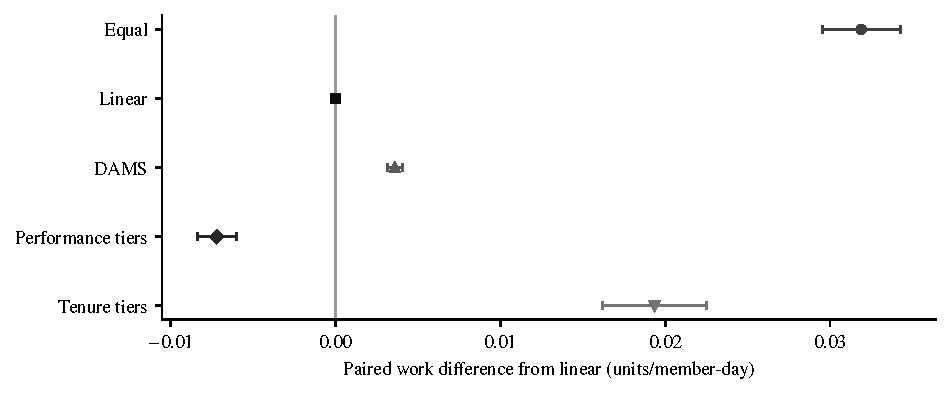
\includegraphics[width=\textwidth]{figures/results/allocation-effects.pdf}
\caption{Allocation effects relative to linear credit in 32 matched independent synthetic worlds. Symbols identify policies; bars are conditional 95\% normal Monte Carlo intervals. Equal baselines and the zero linear contrast are retained. Daily update, central record, 120 members and 60 days; source \texttt{3d67a62e6eb2}.}
\label{fig:allocation-effects}
\end{figure}
\begin{figure}[tbp]
\centering
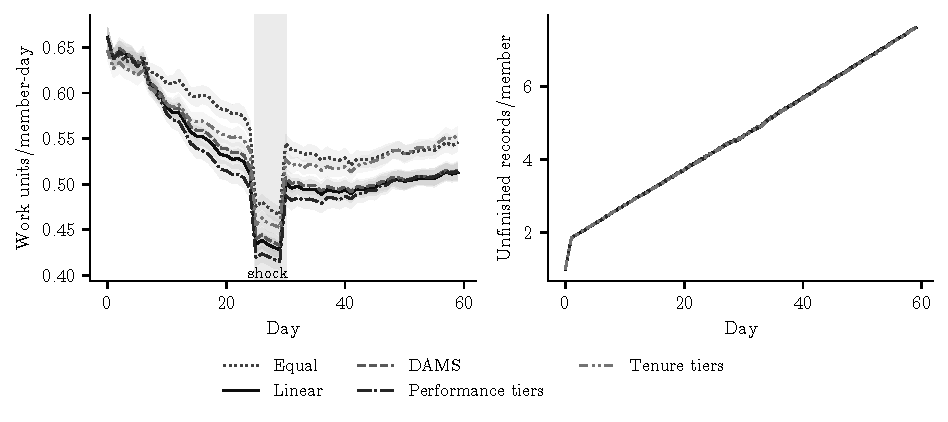
\includegraphics[width=\textwidth]{figures/results/governance-dynamics.pdf}
\caption{Daily generated work and unfinished review/settlement records in the same 32 worlds. Lines are world means and faint bands are pointwise 95\% Monte Carlo intervals; they are not trajectory prediction bands. The shaded site-0 shock lasts days 25--29. No smoothing is applied. The queue stock excludes appeals. DAMS-ABM 0.1.0, source \texttt{3d67a62e6eb2}.}
\label{fig:governance-dynamics}
\end{figure}
\begin{figure}[tbp]
\centering
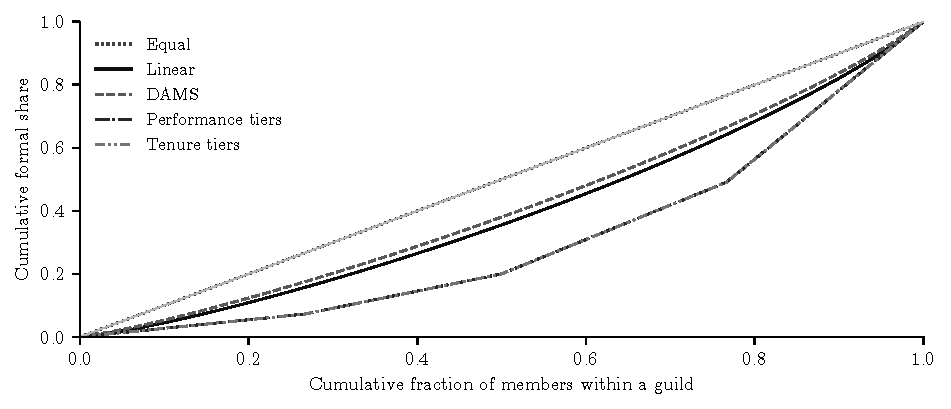
\includegraphics[width=\textwidth]{figures/results/formal-authority-distribution.pdf}
\caption{Final frozen formal-authority distributions for five policies, central record and daily updates. Lorenz curves are averaged across four 30-member guilds within each world and then over 32 independent worlds. Domain rights are not pooled into one organization-wide right. The diagonal indicates equal allocation; greater equality is not evidence of fairness, legitimacy or better decisions. Synthetic source \texttt{3d67a62e6eb2}.}
\label{fig:formal-authority-distribution}
\end{figure}
\begin{table}[tbp]
\centering\small
\caption{Same DAMS policy under three conditional evidence-process settings.}
\label{tab:ledger-stress}
\begin{tabular}{lrrrrr}
\toprule
Record & Work/member-day & Mean days & Unfinished & Review hours & Verify units \\
\midrule
Central & 0.532 & 4.90 & 913 & 637.2 & 0.0 \\
Witness & 0.538 & 10.48 & 2144 & 519.2 & 1038.4 \\
Consensus & 0.544 & 14.98 & 3120 & 424.8 & 2124.0 \\
\bottomrule
\end{tabular}
\par\smallskip\begin{minipage}{0.96\textwidth}\footnotesize 32 independent synthetic worlds per setting. Default cost multipliers and settlement delays are design assumptions, not measured database/log/consensus performance. Human review hours and extra verification units have different units. No monetary or total-cost equivalence is assumed.\end{minipage}
\end{table}
\begin{figure}[tbp]
\centering
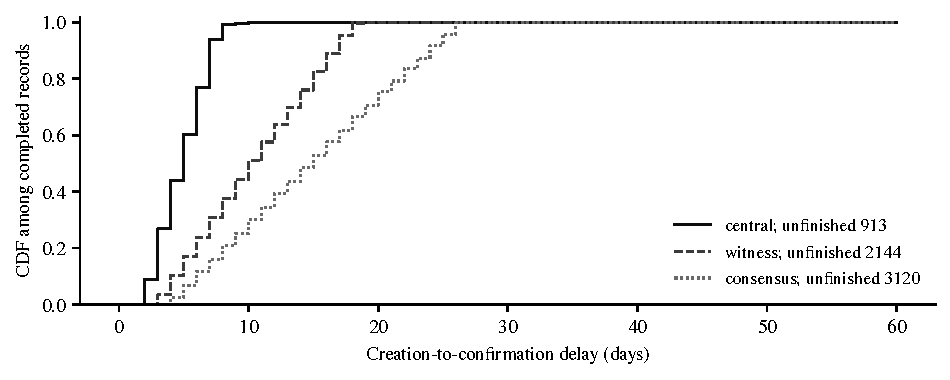
\includegraphics[width=\textwidth]{figures/results/confirmation-cdf.pdf}
\caption{Conditional delay distributions for DAMS under each evidence setting. Curves average the completed-record CDF of 32 independent worlds; legend values are mean unfinished horizon stocks. This is not a survival estimate for all submissions: incomplete records are excluded from each CDF and reported separately. Full integer-day steps are retained to day 60. Synthetic model source \texttt{3d67a62e6eb2}.}
\label{fig:confirmation-cdf}
\end{figure}
\begin{figure}[tbp]
\centering
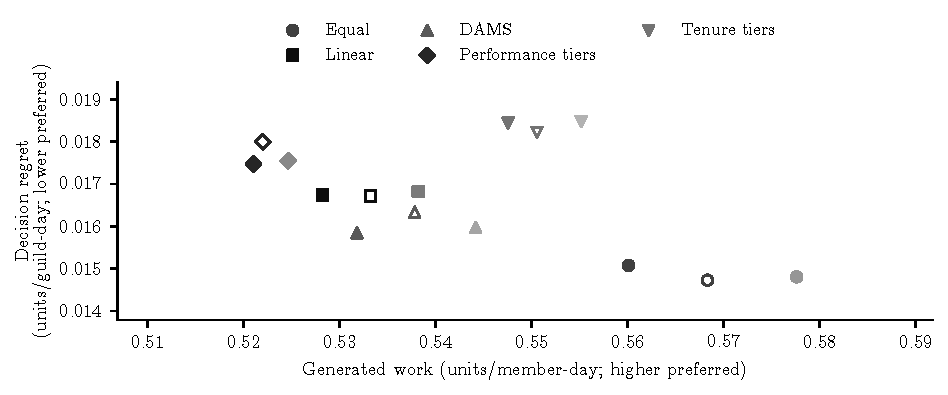
\includegraphics[width=\textwidth]{figures/results/outcome-tradeoffs.pdf}
\caption{Outcome-vector comparison for five policies and three record settings: 32-world means under daily update. Filled symbols denote central, hollow symbols witnessed and lighter filled symbols consensus assumptions. This diagram shows competing modeled objectives without converting them into welfare or money; uncertainty and paired effects are reported separately. A mean-position advantage does not establish universal Pareto dominance.}
\label{fig:outcome-tradeoffs}
\end{figure}
